\paragraph{Network Architecture}~\\
The network architecture we used for the inverse problem contained pooling layers to gradually reduce the many parameters of a spectrum $I$ to a few design parameters $\mc D$. Here we have to go the opposite way and upsample $\mc D$ to $I$. For this we will use upsampling layers which double the size of their input, e.g. $(1,3) \rightarrow (1,1,3,3)$. The convolution is then applied to this upsampled output to "fill in the details" \cite{fill_in_details}. This combination of upsampling and convolution is called \textit{transposed convolution} in literature \cite{TransposedConv}. The full Network architecture is shown in figure \ref{fig:in:NN} and contains two more new layers. Batch Normalization (BN) and a running average filter (Avg).
\\

\indent
Batch Normalization was introduced by Ioffe and Szegedy in 2015 \cite{Ioffe2015}. This layer calculates the mean $\mu_\mc B$ and variance $\sigma_\mc B$ over every \hyperref[hyp:minibatch]{mini-batch} $\mc B$. Then it normalizes the output of the previous layer $\vb x$ to 
\begin{equation}
    \bar x_i = \frac{x_i - \mu_\mc B}{\sigma_\mc B}
    \qq{and rescales it to}
    y_i = \gamma \bar x_i + \beta \,,
\end{equation}

where $\gamma$ and $\beta$ are trainable parameters. This way the output of the previous layer has a mean of zero and a variance of one which has advantages for the networks stability and training speed \cite{Ioffe2015}.
(Batch Normalization was later also added to the inverse model.)
Additionally, the running average filters were added because the output oscillated too much on small wavelength differences.
This way the fact, that transmission spectra do not change too much on a per wavelength scale, is directly contained in the network architecture. 
\\

\begin{figure}[H]
    \centering
    \includegraphics[width=\linewidth]{in_NN_architecture}
    \caption{Network architecture of the forward model. First the discrete and continuous inputs are combined and connected to a Dense layer with 
    $(20 \cdot 128)$
    neurons. The number 20 will later become 160 discretized wavelength after the three upscale operations are applied. As discussed in section \ref{sec:NN_bg} convolutional layers operate on stacked feature maps. This is why the $20 \cdot 128$ flat neurons need to be reshaped into a $20 \times 128$ array. Next there are three transposed convolutional layers $CNU$. Each consisting on a basic convolution $C$, a Batch Normalization $N$ and an upscale layer $U$. The convolution is characterized by the parameters (\textit{number of kernels, kernel size}). The final convolution $C^4$ reduces the number stacked feature maps to 2. One each for the $x$ and $y$ polarization. Finally, two running average filters (Avg) are applied to smooth the output. All the internal activations $\sigma_\s{r}$ are ReLu's and the final activations $\sigma_{l}$ is a linear function.
    Layers which contain trainable parameters are marked red.
    }
    \label{fig:in:NN}
\end{figure}



\newpage
\paragraph{Network Training}~\\
The forward model is trained like the inverse model just the inputs and outputs are exchanged. That is, the training data $(X,\, Y)$ now consists of tuples 
$(\mc D,\, I)$ instead of $(I,\, \mc D)$.
This allows us to use the same underlying data of pre simulated stacks, we already have, to also train the forward model. 
The mean absolute error (mae) per spectrum drops to 0.04 over 20 epochs as shown in figure \ref{fig:in:forward_training}. $I$ consists of 160 discretized wavelengths for two polarizations. This means the transmission at every wavelength is on average $4/320 = 1/30$ percent points off. However, the forward model is not perfect. As can be seen in figure \ref{fig:in:avg_plot} it generates small troughs and peaks where there are none in the original spectrum.
\\

\indent
Now we can combine the inverse model $\mc D \rightarrow I$ and the forward model $I \rightarrow \mc D$ into a combined model $I \rightarrow \mc D \rightarrow I'$ and directly use the loss function $C_\s{mse}(I,\, I')$.
However, even trying different regularization techniques, this model could not be trained successfully as seen in figure \ref{fig:ap:combined_training}.  


\begin{figure}[H]
    \floatbox[{
    \capbeside
    \thisfloatsetup{capbesideposition={right,top}}}]{figure}[\FBwidth]
    {\caption{
        Training of the forward model. The Network performance is evaluated based on the mean absolute error (mae). If $I$ is the real spectrum and $I'$ is the networks output then 
        $C_\s{mae} = \sum_i \qty|I_i - I'_i|$.
    }
    \label{fig:in:forward_training}}
    {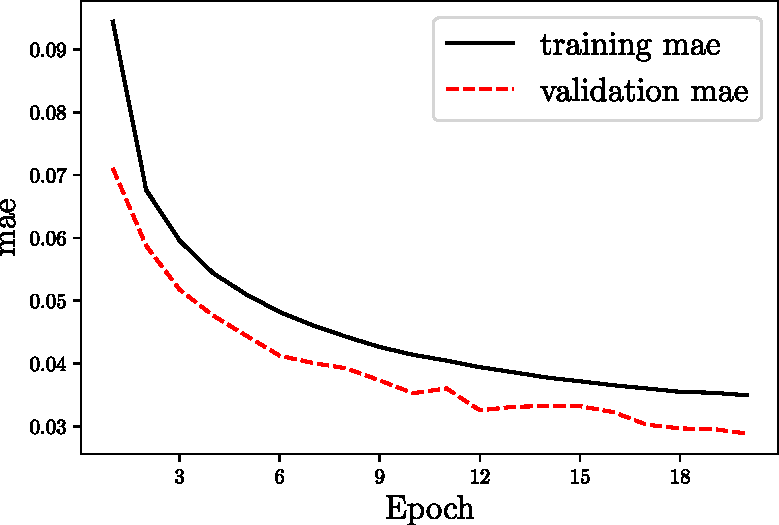
\includegraphics[width=0.6\textwidth]{in_forward_training}}
\end{figure}

\begin{figure}[H]
    \floatbox[{
    \capbeside
    \thisfloatsetup{capbesideposition={right,top}}}]{figure}[\FBwidth]
    {\caption{
        Training of the combined model. Validation loss oscillates wildly.
    }
    \label{fig:ap:combined_training}}
    {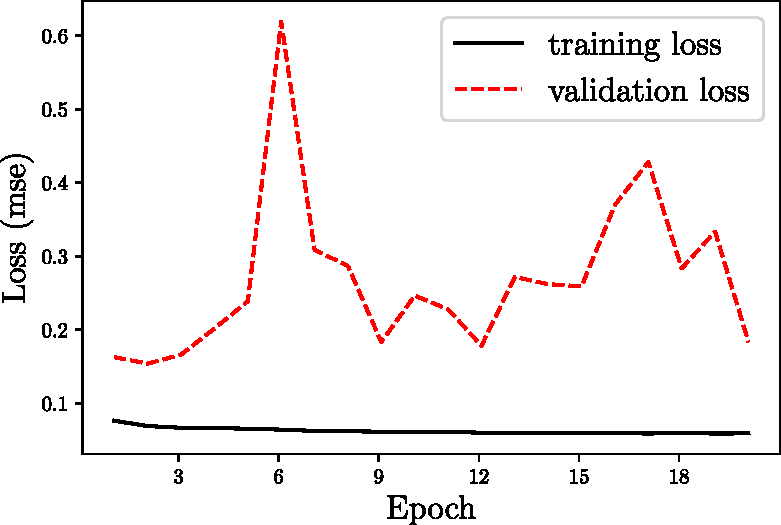
\includegraphics[width=0.6\textwidth]{ap_combo}}
\end{figure}
